% Created by tikzDevice version 0.10.1 on 2018-01-15 11:47:04
% !TEX encoding = UTF-8 Unicode
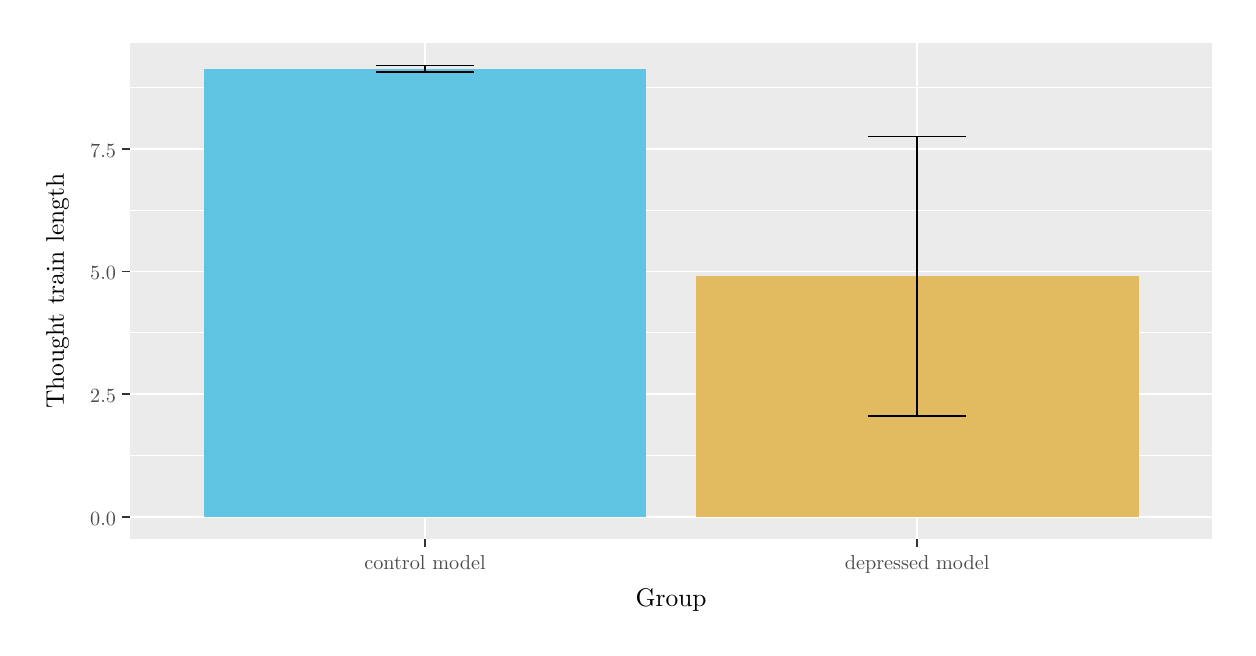
\begin{tikzpicture}[x=1pt,y=1pt]
\definecolor{fillColor}{RGB}{255,255,255}
\path[use as bounding box,fill=fillColor,fill opacity=0.00] (0,0) rectangle (433.62,216.81);
\begin{scope}
\path[clip] (  0.00,  0.00) rectangle (433.62,216.81);
\definecolor{drawColor}{RGB}{255,255,255}
\definecolor{fillColor}{RGB}{255,255,255}

\path[draw=drawColor,line width= 0.6pt,line join=round,line cap=round,fill=fillColor] (  0.00,  0.00) rectangle (433.62,216.81);
\end{scope}
\begin{scope}
\path[clip] ( 36.87, 31.92) rectangle (428.12,211.31);
\definecolor{fillColor}{gray}{0.92}

\path[fill=fillColor] ( 36.87, 31.92) rectangle (428.12,211.31);
\definecolor{drawColor}{RGB}{255,255,255}

\path[draw=drawColor,line width= 0.3pt,line join=round] ( 36.87, 62.22) --
	(428.12, 62.22);

\path[draw=drawColor,line width= 0.3pt,line join=round] ( 36.87,106.52) --
	(428.12,106.52);

\path[draw=drawColor,line width= 0.3pt,line join=round] ( 36.87,150.83) --
	(428.12,150.83);

\path[draw=drawColor,line width= 0.3pt,line join=round] ( 36.87,195.13) --
	(428.12,195.13);

\path[draw=drawColor,line width= 0.6pt,line join=round] ( 36.87, 40.07) --
	(428.12, 40.07);

\path[draw=drawColor,line width= 0.6pt,line join=round] ( 36.87, 84.37) --
	(428.12, 84.37);

\path[draw=drawColor,line width= 0.6pt,line join=round] ( 36.87,128.68) --
	(428.12,128.68);

\path[draw=drawColor,line width= 0.6pt,line join=round] ( 36.87,172.98) --
	(428.12,172.98);

\path[draw=drawColor,line width= 0.6pt,line join=round] (143.57, 31.92) --
	(143.57,211.31);

\path[draw=drawColor,line width= 0.6pt,line join=round] (321.41, 31.92) --
	(321.41,211.31);
\definecolor{fillColor}{RGB}{95,197,226}

\path[fill=fillColor] ( 63.54, 40.07) rectangle (223.60,202.02);
\definecolor{fillColor}{RGB}{226,186,95}

\path[fill=fillColor] (241.39, 40.07) rectangle (401.44,126.99);
\definecolor{drawColor}{RGB}{0,0,0}

\path[draw=drawColor,line width= 0.6pt,line join=round] (125.79,203.16) --
	(161.36,203.16);

\path[draw=drawColor,line width= 0.6pt,line join=round] (143.57,203.16) --
	(143.57,200.89);

\path[draw=drawColor,line width= 0.6pt,line join=round] (125.79,200.89) --
	(161.36,200.89);

\path[draw=drawColor,line width= 0.6pt,line join=round] (303.63,177.54) --
	(339.20,177.54);

\path[draw=drawColor,line width= 0.6pt,line join=round] (321.41,177.54) --
	(321.41, 76.45);

\path[draw=drawColor,line width= 0.6pt,line join=round] (303.63, 76.45) --
	(339.20, 76.45);
\end{scope}
\begin{scope}
\path[clip] (  0.00,  0.00) rectangle (433.62,216.81);
\definecolor{drawColor}{gray}{0.30}

\node[text=drawColor,anchor=base east,inner sep=0pt, outer sep=0pt, scale=  0.73] at ( 31.92, 37.04) {0.0};

\node[text=drawColor,anchor=base east,inner sep=0pt, outer sep=0pt, scale=  0.73] at ( 31.92, 81.34) {2.5};

\node[text=drawColor,anchor=base east,inner sep=0pt, outer sep=0pt, scale=  0.73] at ( 31.92,125.64) {5.0};

\node[text=drawColor,anchor=base east,inner sep=0pt, outer sep=0pt, scale=  0.73] at ( 31.92,169.95) {7.5};
\end{scope}
\begin{scope}
\path[clip] (  0.00,  0.00) rectangle (433.62,216.81);
\definecolor{drawColor}{gray}{0.20}

\path[draw=drawColor,line width= 0.6pt,line join=round] ( 34.12, 40.07) --
	( 36.87, 40.07);

\path[draw=drawColor,line width= 0.6pt,line join=round] ( 34.12, 84.37) --
	( 36.87, 84.37);

\path[draw=drawColor,line width= 0.6pt,line join=round] ( 34.12,128.68) --
	( 36.87,128.68);

\path[draw=drawColor,line width= 0.6pt,line join=round] ( 34.12,172.98) --
	( 36.87,172.98);
\end{scope}
\begin{scope}
\path[clip] (  0.00,  0.00) rectangle (433.62,216.81);
\definecolor{drawColor}{gray}{0.20}

\path[draw=drawColor,line width= 0.6pt,line join=round] (143.57, 29.17) --
	(143.57, 31.92);

\path[draw=drawColor,line width= 0.6pt,line join=round] (321.41, 29.17) --
	(321.41, 31.92);
\end{scope}
\begin{scope}
\path[clip] (  0.00,  0.00) rectangle (433.62,216.81);
\definecolor{drawColor}{gray}{0.30}

\node[text=drawColor,anchor=base,inner sep=0pt, outer sep=0pt, scale=  0.73] at (143.57, 20.91) {control model};

\node[text=drawColor,anchor=base,inner sep=0pt, outer sep=0pt, scale=  0.73] at (321.41, 20.91) {depressed model};
\end{scope}
\begin{scope}
\path[clip] (  0.00,  0.00) rectangle (433.62,216.81);
\definecolor{drawColor}{RGB}{0,0,0}

\node[text=drawColor,anchor=base,inner sep=0pt, outer sep=0pt, scale=  0.92] at (232.49,  7.83) {Group};
\end{scope}
\begin{scope}
\path[clip] (  0.00,  0.00) rectangle (433.62,216.81);
\definecolor{drawColor}{RGB}{0,0,0}

\node[text=drawColor,rotate= 90.00,anchor=base,inner sep=0pt, outer sep=0pt, scale=  0.92] at ( 13.08,121.61) {Thought train length};
\end{scope}
\end{tikzpicture}
